O objetivo principal do agente de \textit{MM} é decidir dentro do intervalo de preços possíveis para uma ação o valor que proporcione o maior retorno para o menor risco associado, de acordo com a fronteira eficiente de execução ótima \citep{almgren2000}. O agente também pode decidir a quantidade de ações ofertadas por determinado preço, mas não tem controle direto sobre as quantidades efetivamente negociadas. Ou seja, a quantidade executada $q$ é uma variável aleatória, dado que não é possível determinar de antemão quanto o agente agressor irá negociar com o agente de \textit{market-making}. Sabe-se apenas que a quantidade negociada é menor ou igual à ofertada ($q \leq Q$). 

Podemos consequentemente modelar o agente como um problema de otimização estocástica com restrições, onde o objetivo inicial do agente é separado em duas etapas: 

\begin{enumerate}[]
	\item maximização do \textit{bid-ask spread} $\mathbf{\Delta}_{t,i} = \delta_{t, i}(p^{a}) + \delta_{t, i}(p^{b}) = |p^{a} - p^{b}|$  para todos ativos;
	
	\item maximização da quantidade executada esperada $\mathbb{E} [q_{t, i}^{a}]$ e $\mathbb{E} [q_{t, i}^{b}]$ de ordens de venda e compra realizadas em cima do maior \textit{bid-ask spread} $\mathbf{\Delta}_{t, i}$, garantindo que a negociação ocorra na fronteira eficiente de execução.
\end{enumerate}

As variáveis de decisão são as combinações possíveis de ofertas de venda e compra — ou seja, o conjunto de combinações de pares de preços e quantidades ofertadas $o_{t}$\footnote{\ Note que o agente decide a quantidade ofertada $Q$, e não tem controle direto sobre a quantidade executada $q$, pois é uma variável aleatória.} (em termos computacionais, $o_{t}$ é usualmente representado por uma lista de tuplas representando as ofertas):
\begin{equation}
	o_{t} = \{(p_{t, 0}^{a}, Q_{t, 0}^{a}), ..., (p_{t, n}^{a}, Q_{t, n}^{a}), (p_{t, 0}^{b}, Q_{t, 0}^{b}), ..., (p_{t, m}^{b}, Q_{t, m}^{b})\}
\end{equation} A função objetivo do problema é o valor esperado do retorno diário, considerando a incerteza da quantidade executada $q_{t, i} \leq Q_{t, i}$ por ordem. Substituindo o valor de $q$ na equação (\ref{return}) pelo seu valor esperado:

\begin{equation}
	\begin{aligned}
		\mathbb{E} [r_{t}] = 
		\sum_{i = 0}^{n} \delta_{t}(\ p_{t, i}^{a}\ ,\ \mathbb{E} [\ q_{t, i}^{a}\ ]) \\
		-\sum_{i = 0}^{m} \delta_{t}(\ p_{t, i}^{b}\ ,\ \mathbb{E} [\ q_{t, i}^{b}\ ]) \\
		\forall t < T
	\end{aligned}
\end{equation}

e o retorno diário acumulado da equação \ref{return_accumulated} é utilizado como função objetiva que se deseja maximizar em relação à variável $o$ de ofertas do agente:
\begin{equation} \label{objective_equation}
	\begin{aligned}
		\max_{o} \quad & \mathbb{E} [\sum_{t=0}^{T} \ r_{t}]
	\end{aligned}
\end{equation}

De modo a obter uma solução para a otimização estocástica definimos o agente como um processo de decisão de Markov $(\mathcal{S}, \mathcal{A}, T, r)$, buscando modelar o problema para o paradigma de Aprendizado por Reforço:

\begin{description}
	\item[$\mathcal{S}$] 
	é o espaço de estados possíveis, representado pelo conjunto $\{o_{t}, L_{t}) \ | \ t < T\}$, onde cada estado $s \in \mathcal{S}$ é uma combinação possível de ofertas do agente $o$, e a observação do livro de ordens limite $L$ no momento $t$;
	
	\item[$\mathcal{A}$] é o espaço de ações que o agente pode realizar, ou seja, a combinação de preços $p_{t + 1}$ e novas quantidades $Q_{t+1}$ para cada tupla $(p_{t}, Q_{t})$ do conjunto $o_{t}$ de ofertas de venda e compra existentes;
	
	\item[\textit{T}] são as transições possíveis entre estados dado uma ação tomada pelo agente. São representadas pela função de transição $T :  \mathcal{S} \times \mathcal{A} \times \mathcal{S} \rightarrow [0, 1]$, que mapeia o estado atual e a ação tomada para a probabilidade de ir para um estado subjacente. No caso do agente de \textit{market-making}, a função $T$ recebe o estado atual $s$ e a ação $a$ tomada pelo agente (conjunto de \textit{spreads} e quantidades ofertadas atualizadas). Em seguida recebe um possível estado futuro $s' \in \mathcal{S}$ e retorna a probabilidade de transição $T(s, a, s') = Pr(S_{t+1} = s' \ | \ S_{t} = s, A = a)$. O valor dessa função não é conhecido a não ser para sistemas muito simples, o que requer o uso de técnicas de programação dinâmica ou aprendizado por reforço para estimar a sua distribuição, como o método tabular \textit{Q-Learning} e \textit{Proximal Policy Optimization};
+++	
	\item[\textit{r}] é a função de recompensa da cadeia aleatória, que mapeia o estado atual e a ação do agente para a probabilidade de uma recompensa ocorrer caso a transição para um determinado estado seguinte ocorra. No caso do agente de \textit{MM}, a função de recompensa é o próprio retorno $r_{t+1}$ do agente.
\end{description}

\begin{figure}[H]
	\centering
	\documentclass[tikz,border=10pt]{standalone}
\usepackage{pgf}
\usepackage{xcolor}

\begin{document}
	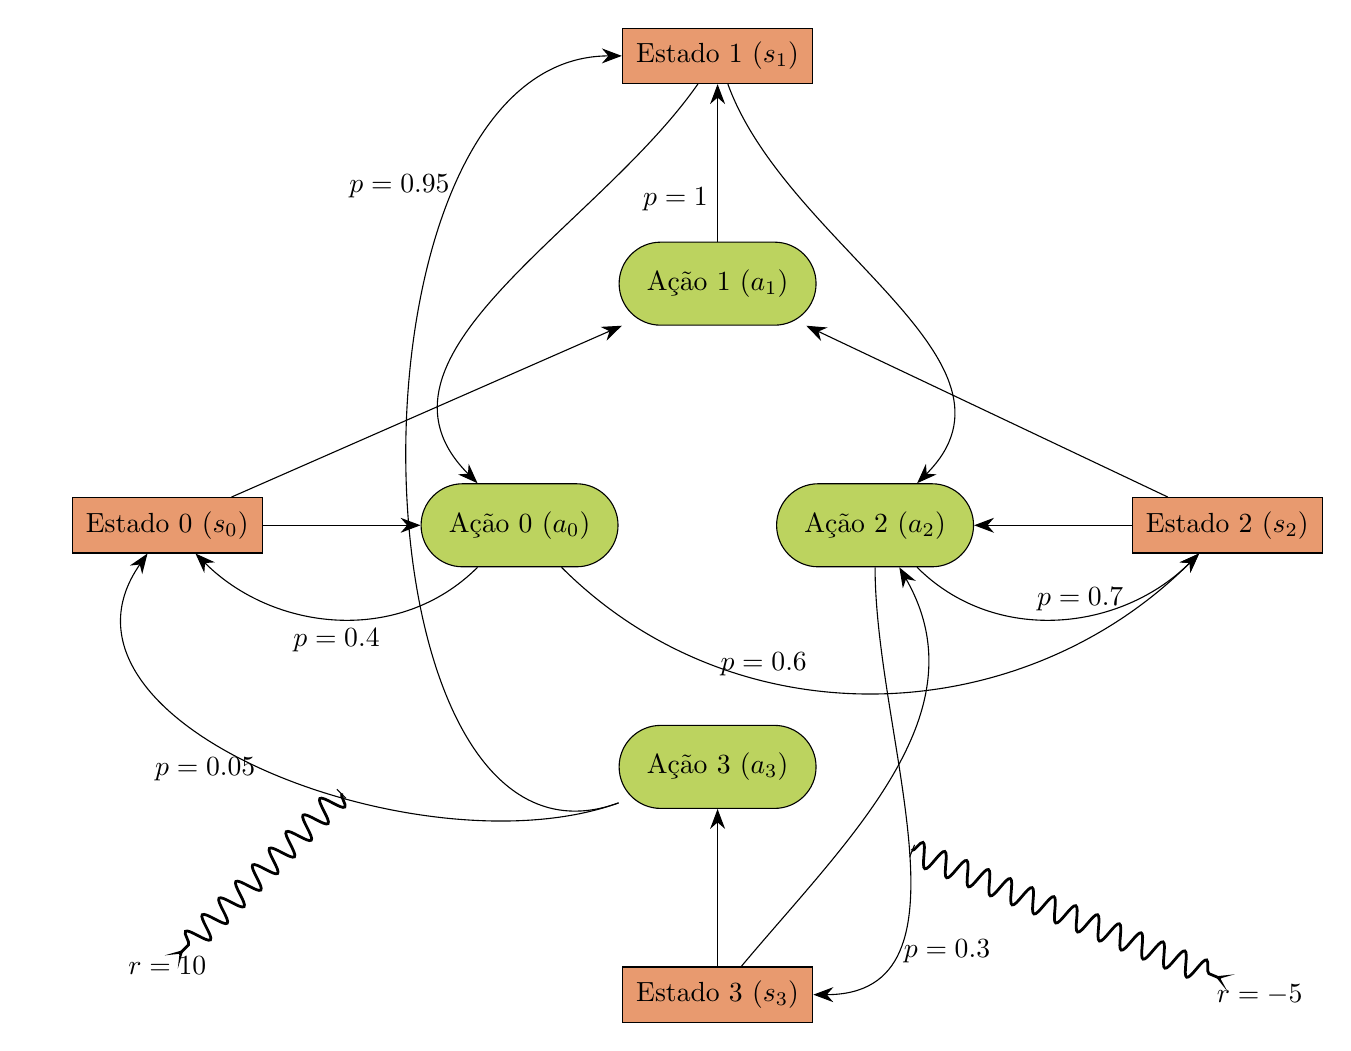
\begin{tikzpicture}
		\usetikzlibrary{arrows,automata,positioning,arrows.meta};
		\definecolor{statecolor}{HTML}{e89a6f};
		\definecolor{actioncolor}{HTML}{bcd35f};
		\tikzset{
			state/.style={
				shape=rectangle,
				draw=black,
				fill=statecolor,
				align=center,
				minimum height=2em,
				minimum width=4em,
				inner sep=5pt,
			},
			action/.style={
				shape=rectangle,
				draw=black,
				fill=actioncolor,
				align=center,
				inner sep=10pt,
				rounded corners=15pt,
			},
			reward/.style={
				|-,
				decoration={snake, amplitude=1.5mm, segment length=3mm},
				decorate,
				postaction={draw, line width=1pt, -{Stealth[scale=-0.8]}}
			},
			transition/.style={
				->,
				>={Stealth[scale=1.5]},
			}
		};
		\tikzset{node distance=2cm and 2cm}
    	\node[state] (s0) {Estado 0 ($s_0$)};

		\node[action, right=2cm of s0] (a0) {Ação 0 ($a_0$)};
		\node[action, above right=2cm and 0cm of a0] (a1) {Ação 1 ($a_1$)};
		\node[action, right=2cm of a0] (a2) {Ação 2 ($a_2$)};
		\node[action, below right=2cm and 0cm of a0] (a3) {Ação 3 ($a_3$)};

		\node[state, above=2cm of a1] (s1) {Estado 1 ($s_1$)};
		\node[state, right=2cm of a2] (s2) {Estado 2 ($s_2$)};
		\node[state, below=2cm of a3] (s3) {Estado 3 ($s_3$)};
		
		\node[draw=none, below right=2.8cm and 1cm of s0] (r0s) {};
		\node[draw=none, below=5cm of s0] (r0e) {$r=10$};
		
		\node[draw=none, above right=1.4cm and 1cm of s3] (r1s) {};
		\node[draw=none, right=5cm of s3] (r1e) {$r=-5$};
		
		\begin{scope} % actions
			\draw[transition] 
			(s0) 
			to
			(a0);
	
			\draw[transition] 
			(s0) 
			to
			(a1);
	
			\draw[transition] 
			(s1) 
			to[in=45, out=290]
			(a2);
	
			\draw[transition] 
			(s1) 
			to[in=135, out=235]
			(a0);
	
			\draw[transition] 
			(s2) 
			to
			(a1);
	
			\draw[transition] 
			(s2) 
			to
			(a2);
	
			\draw[transition] 
			(s3) 
			to
			(a3);
	
			\draw[transition] 
			(s3) 
			to[in=300, out=50]
			(a2);		
		\end{scope}
		
		\begin{scope} % transitions
			\draw[transition] 
			(a0)
			to[in=315, out=225] node[midway, below] 
			{$p = 0.4$} 
			(s0);
			
			\draw[transition] 
			(a0) 
			to[in=225, out=315] node[near start, right] 
			{$p = 0.6$} 
			(s2);
			
			\draw[transition] 
			(a1) 
			to[in=270, out=90] node[near start, left] 
			{$p = 1$} 
			(s1);
			
			\draw[transition] 
			(a2) 
			to[in=225, out=315] node[near end, left] 
			{$p = 0.7$} 
			(s2);
			
			\draw[transition] 
			(a2) 
			to[in=0, out=270] node[near end, right] 
			{$p = 0.3$} 
			(s3);
			
			\draw[transition] 
			(a3) 
			to[in=235, out=200] node[midway, left] 
			{$p = 0.05$} 
			(s0);
			
			\draw[transition] 
			(a3) 
			to[in=180, out=200] node[near end, left] 
			{$p = 0.95$} 
			(s1);
		\end{scope}
		
		\begin{scope}
			\draw[reward]
			(r0s)
			to
			(r0e);
			
			\draw[reward]
			(r1s)
			to
			(r1e);
			
		\end{scope}
	\end{tikzpicture}
\end{document}

	\caption{Processo de Decisão de Markov com 4 estados e ações (MDP)}
	\label{fig:mdp}
\end{figure}

Utilizando a definição do agente como um Processo de Decisão de Markov, podemos simular o ambiente e encontrar uma política de decisão de preços ótimas. As técnicas de Aprendizado por Reforço serão usadas para essa tarefa, e abaixo o problema inicial de otimização do agente será traduzido à notação usada na área de \textit{RL} que parte das \textit{MDPs} de modo a permitir o uso de algoritmos computacionais de otimização para \textit{market making}.


\begin{itemize}
	\item Trajetória ($\tau$): é a sequência de estados observados e ações tomadas ao longo do tempo. No contexto de \textit{MM}, uma trajetória consiste em uma série de estados do mercado $s_{t} = (o_{t}, L_{t})$ seguidas da ação em cima desse estado $a_{t} = \{(\delta_{t}(p_{i}), Q_{i}) \ | \ \forall i \}$. Essas trajetórias representam a jornada do agente no mercado financeiro, incluindo suas ações e interações com o ambiente.
	
	\[
	\tau = (s_0, a_0, s_1, a_1, \ldots, s_T, a_T)
	\]
	
	Onde \(s_t\) é o estado no tempo \(t\), e \(a_t\) é a ação tomada no tempo \(t\).
	
	\item Política ($\pi$): função que mapeia o estado atual (\textit{spreads} $\delta$ e quantidades $Q$) para a escolha de ações (ofertas de compra e venda). Através de algoritmos de otimização de decisão (\textit{Policy Optimization} e \textit{Q-Learning}), nosso objetivo é encontrar uma política ótima que permita ao agente tomar decisões que maximizem seus retornos no mercado. Essa política é fundamental para determinar como o agente se comporta em diferentes situações de mercado.
	
	\[
	\pi(s) \rightarrow a
	\]
	
	Essa função determina como o agente toma decisões em diferentes estados.
	
	\item Função de Valor ($V$): estima o valor esperado acumulado que o agente pode obter ao seguir a política \(\pi\) a partir de um estado inicial. No contexto do agente de \textit{market making}, $V$ depende do preço de venda $p$ e da quantidade $q$ executada, bem como da política do agente. Através do Aprendizado por Reforço, podemos calcular \(V\) para avaliar quão bom é um estado, o que orienta o agente na seleção de ações que maximizam seu desempenho global.
	
	\begin{equation*}
		V(s_0) = \mathbb{E}\left[\sum_{t=0}^{T} \gamma^t \cdot r(s_t, \pi(s_t)) \right]
		\end{equation*}
	
	Onde $\gamma$ é o fator de desconto que pondera as recompensas futuras e geralmente $0 < \gamma \leq 1$. A função valor considera a expectativa de retorno sobre todas as possíveis trajetórias do agente.
\end{itemize}

\begin{figure}[H]
	\centering
	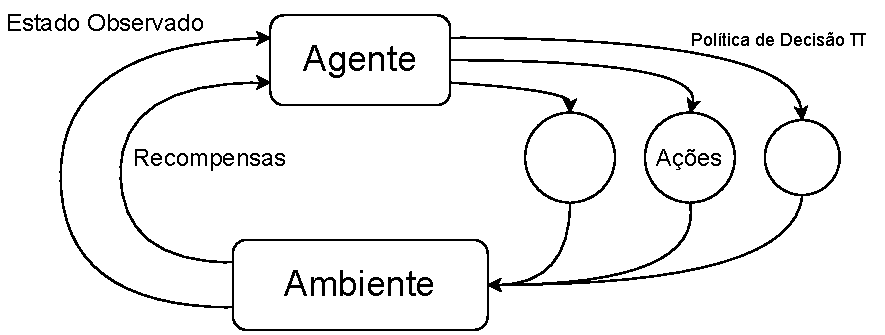
\includegraphics{files/rl-agent.pdf}
	\caption{Autômato do Agente sob o paradigma de Aprendizado por Reforço}
	\label{fig:rl-agent}
\end{figure}

O agente passa a ser representado pela nova tupla $(V, \tau, \pi)$ onde $V$ e $\tau$ são dadas pelo processo $\mathbf{MDP}$. O paradigma de Aprendizado por Reforço permite que o agente se adapte a mudanças nas condições de mercado ao longo do tempo, e que a política escolhida considere o impacto das transações do próprio agente sobre o mercado, tornando-o mais resiliente a flutuações causadas pelas próprias ações. Uma vez treinado, o agente pode ser usado para tomar decisões em tempo real no mercado financeiro, proporcionando uma vantagem competitiva para instituições financeiras e o avanço da pesquisa em finanças quantitativas e aprendizado de máquina, abrindo novas possibilidades para o desenvolvimento de estratégias de negociação mais eficientes e robustas. A contribuição da pesquisa proposta será tornar o agente adverso ao risco noturno, inserindo-se também uma restrição adicional, de que ao final do dia não haja exposição a riscos de mercado. 
Existem algumas alternativas para formalizar matematicamente essa restrição:
\begin{enumerate}
    \item No final do dia, o agente não pode ter nenhum ativo em posição: 
    \begin{equation} \label{overnight_restriction}
        \sum_{i = 0}^{n} q_{T, i}^{a}  = \sum_{i=0}^{m} q_{T, i}^{b} = 0
    \end{equation}
    \item No final do dia, se houver alguma posição restante, o agente precisa \textit{headgear}\footnote{De maneira simplificada, o \textit{hedge} consiste em comprar ou vender ativos que tenham uma exposição ao risco oposta aos riscos da carteira atual, de modo a equilibrar a posição.} sua exposição ao risco ao participar em outros mercados abertos no momento, abordagem que chamamos de \textit{market making} \textbf{simultâneo}.
\end{enumerate}
